\section{Build pipelines}
\label{sec:buildpipelines}

%% Graphic of build pipeline components
\begin{figure} % h-ere, t-op, b-ottom, p-age
    \centering
    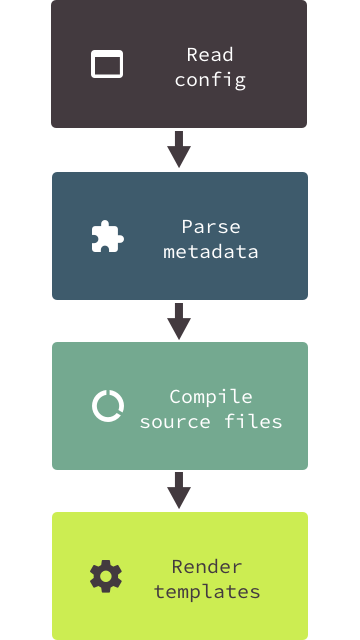
\includegraphics[width=0.9\textwidth]{build_pipeline.png}
    \caption{A graphic showing the basic flow of a \emph{build pipeline}.\\
    First, the configuration file is read and necessary modules invoked. Second, the global metadata, as well as metadata from within the content, is parsed and stored in the global configuration. Third, the content sources get compiled into basic \emph{HTML} markup. Last, the compiled content gets rendered into predefined templates, to apply a given structure which is used commonly throughout the website.}
    \label{fig:build-pipeline}
\end{figure}
%

A static site generator mostly consists of a build pipeline, which handles the workflow needed for bringing the content into shape. This goes from setting the boundaries, determined by a configuration file, to finally producing a web root, consisting of HTML, CSS and JavaScript files, as well as images.

Normally, the major part of it happens sequentially, as nearly all content files are facing a series of transformations on them \cite{Metalsmith2015technicaldocumentation}. Although the amount and extent of conversions may differ significantly from pipeline setup to pipeline setup, it can be broken down to the following core parts (see fig. \ref{fig:build-pipeline}):

\begin{description}
  \item[Metadata parser] -- Parses global metadata, found in the configuration file or in the YAML frontmatter of content files.
  \item[Markdown compiler] -- Used to convert easily read- and writeable Markdown files in browser-readable HTML.
  \item[Template renderer] -- Responsible for bringing the very basic content structure in shape. The goal should be a common appearence, enriched with additional elements (like navigation, breadcrumbs, \ldots).
\end{description}

Of course, the list above overlaps at some point with the list mentioned in <<\emph{\nameref{par:creatingcontent}}>> on p. \pageref{par:creatingcontent}, as a build pipeline may be considered only as a part of the given static site generator (although the main part), not as the generator itself. One of the reasons is its independence of programming languages: A build pipeline doesn't care which programming language it consists of, as long as it knows how to interpret the content sources and templates. Therefore, it merely should be called a concept, not a framework.

%% Say something about the config file, yadda yadda yadda one hand pure build pipeline, because of metadata and configuration, other hand no, because of plugins. plugins??

\subsection{Frontmatter}
\label{sec:buildpipelines-frontmatter}

\lstinputlisting[caption={frontmatter.md}, label={list:frontmatter}]{chapters/03-technical-foundations/_support/frontmatter.md}

listing \ref{list:frontmatter} shows a sample usage of frontmatter inside a Markdown file. Bounded by three dashes above the main content source, it allows certain per-file metadata definitions, which will be parsed at build time and provided for the template rendering engine.
% Mention something about omitting databases using frontmatter meta

As an example, the selected template for this sample file may also hold a list for the mentioned \emph{tags}, as well as a placeholder for the \emph{author}'s name and/or \emph{title}. The main content gets then rendered into the respective placeholding tag, already self-containing a basic structure.

Using a \emph{template: false} declaration, some plugins may prevent rendering the content into a template. This might be interesting in cases, where different partials should be included in the DOM by some sort of asynchronous JavaScript later on.


% TODO: Ugly, remove if not necessary anymore, cares for vertical spaces above subsections
\vspace{20pt}

\subsection{Markdown}
\label{sec:buildpipelines-markdown}

\lstinputlisting[caption={markdown.md}, label={list:markdown-demo}]{chapters/03-technical-foundations/_support/markdown.md}

\texttt{Markdown} consists of shorthand conventions, which should be easier to type for content creators  \cite[38]{dhillon2016}.
Therefore, it makes understanding \texttt{HTML} not a necessary precondition anymore, as a basic content structure may be easily achieved when prepending/surrounding text with certain special characters like \texttt{\#, *, \_, \ldots} (See Listing \ref{list:markdown-demo}).

Originally created by \emph{John Gruber}\footnote{\url{http://daringfireball.net/projects/markdown/} -- Markdown website.} as a plugin for \emph{Movable Type} and \emph{Blosxom} blogging engines \cite{Markdown2004introduction} in March 2004, it should be a supportive tool for users against the complexity of formal markup languages (e.g. \texttt{HTML5}) \cite[4]{RFC7764}. According to \emph{Gruber's} intention, there is no ``invalid'' \texttt{Markdown}, as he suggests the author should either ``keep on experimenting'' or ``change the processor'', if the output happens to fail his/her expectations \cite[5]{RFC7764}.

\texttt{GitHub} finally adapted \texttt{Markdown} to its own version, called ``GitHub Flavored Markdown'' (\emph{GFM}). The people behind it enhanced its original functions to also support \emph{code blocks, tables, strike-through text}, as well as \emph{auto-linking} URL structures in the content \cite[18]{RFC7764}. Additionally, also \texttt{GitHub}-specific functions, such as \emph{user mentions, commit references} or \emph{emojis}, may be used\footnote{\url{https://guides.github.com/features/mastering-markdown/\#GitHub-flavored-markdown} -- GitHub Flavored Markdown cheat sheet on \texttt{GitHub}.}.

Since then, \texttt{GitHub} renders browser-friendly versions of general descriptions written in \texttt{Markdown}, for providing fast and easy overviews of the respective repository. As an example, an existing \texttt{README.md} always appears below the root file tree section on a repository front page \cite[5]{gandrud2013github}.


% TODO: Ugly, remove if not necessary anymore, cares for vertical spaces above subsections
\vspace{20pt}

\subsection{Templates}
\label{sec:buildpipelines-templates}

\emph{Templates} are the frames of each content page, caring for a common, browser-readable HTML structure. A uniform design layout allows site-wide look and feel using a global CSS style sheet, as well as certain events triggered by user behaviour, handled by a single JavaScript file.

Born out of the need to fail-safe produce HTML on the server, as the produced data chunks -- initiated by a client HTTP request -- steadily grew, the goal behind templating engines is primarily to separate business logic from data display. Ideally, at the end of the day, there should be no code in HTML, and no HTML in code \cite[225]{Parr2004templates}.

\begin{program}
  \caption{post.hbs}
  \label{list:handlebars}
\lstinputlisting[language=HTML]{chapters/03-technical-foundations/_support/post.html}
\end{program}

A simple template file example for a blog post is shown in Program \ref{list:handlebars}. It is written in \emph{Handlebars}, a very basic templating language, offering only a very limited amount of template logic. Included are \emph{loops, if/else, partials,~\ldots}~--~however, additional ``\emph{helper}''-functions may be added by the developer.

Although such template logic may come in handy for the most part, as some business logic decisions seem to be rather taken during rendering, instead of being hard-coded before, the concept of data separation is therefore often unknowingly violated \cite[228]{Parr2004templates}. Thus, the choice of the ``optimal'' templating engine for a given project is crucial, as different engines offer a different range of built-in logic. This could go from very conservative \emph{Mustache}\footnote{\url{https://mustache.github.io/} -- Mustache website.} to very powerful ones like \emph{Liquid}\footnote{\url{https://help.shopify.com/themes/liquid} -- Shopify's Liquid template engine.} (see Sec. \ref{sec:jekyll-technology}) or \texttt{EJS}\footnote{\url{http://www.embeddedjs.com/} -- Embedded JavaScript website}.

